\chapter{Diseño y Cálculo Analítico}
\label{sec.c5:diseno_teorico}

\section{Selección de componentes activos}
\label{sec.c5:seleccion_activos}

Para la implementación del circuito se seleccionaron los siguientes dispositivos:
\begin{enumerate}
    \item \textbf{Regulador Integrado LM7812:} Regulador lineal positivo fijo de tres terminales. De acuerdo a la
    consigna, se adopta la versión en encapsulado metálico TO-3 (sufijo K), caracterizado por una resistencia
    térmica juntura-carcasa reducida ($\theta_{jc} \approx \SI{4}{\celsius/\watt}$ frente a los
    $\SI{5}{\celsius/\watt}$ del encapsulado plástico TO-220), lo que optimiza la transferencia de calor hacia el
    disipador común \cite{ti_lm78xx}.
    \item \textbf{Transistor de paso de potencia $Q_1$ (MJ2955):} Se seleccionó el transistor PNP de potencia
    MJ2955, complementario del 2N3055, provisto en encapsulado hermético TO-3. Admite una corriente continua de
    colector de hasta $\SI{15}{\ampere}$, una tensión colector-emisor máxima $V_{CEO} = \SI{60}{\volt}$ y una
    potencia máxima disipable $P_D = \SI{150}{\watt}$ a $T_C = \SI{25}{\celsius}$ \cite{onsemi_mj2955}.
    \item \textbf{Transistor sensor de sobrecarga $Q_2$ (BC557B):} Transistor bipolar PNP de pequeña señal en
    encapsulado TO-92 ($V_{CEO} = \SI{45}{\volt}$, $I_{Cmax} = \SI{100}{\milli\ampere}$, $h_{FE} \approx 200$--$450$).
    Su función es monitorear la caída sobre el resistor sensor y actuar sobre la base de $Q_1$.
\end{enumerate}

\section{Tensión de entrada no regulada $V_{in}$}
\label{sec.c5:vin}

El regulador LM7812 exige una tensión diferencial mínima entre entrada y salida ($V_{drop}$) de entre
$\SI{2}{\volt}$ y $\SI{2.5}{\volt}$ para sostener la regulación interna en su zona activa. A esta caída debe
sumarse la tensión en el resistor exterior de disparo $R_{ext}$ ($\approx \SI{0.7}{\volt}$). En consecuencia:
\begin{align*}
    V_{in(min)} &\ge V_{out} + V_{drop} + V_{Rext} \\
    V_{in(min)} &\ge \SI{12}{\volt} + \SI{2.5}{\volt} + \SI{0.7}{\volt} = \SI{15.2}{\volt}
\end{align*}
Adoptamos como tensión de entrada nominal continua $V_{in} = \SI{18}{\volt}$. Esta elección proporciona un margen
de seguridad dinámico de casi $\SI{3}{\volt}$ sobre el límite de dropout, garantizando que variaciones de línea
del $\pm 10\%$ ($16.2\text{ V} \le V_{in} \le 19.8\text{ V}$) no provoquen abandono de regulación.

\section{Cálculo de resistores del elevador y protección}
\label{sec.c5:calculo_resistores}

\subsection{Resistor de disparo del transistor de paso ($R_{ext}$ / $R_2$)}
El resistor $R_{ext}$ conecta el riel de entrada no regulado con la entrada del integrado y la base de $Q_1$. A bajas
corrientes de carga, el transistor $Q_1$ permanece cortado y la totalidad de la corriente circula por el LM7812.
Para que $Q_1$ comience a conducir cuando la corriente del regulador alcance un umbral seguro
$I_{reg(th)} \approx \SI{580}{\milli\ampere}$, se dimensiona:
\begin{equation}
    R_{ext} = \frac{V_{BE(Q1)}}{I_{reg(th)}} = \frac{\SI{0.7}{\volt}}{\SI{0.58}{\ampere}} \approx \SI{1.2}{\ohm}
    \label{eq.c5:rext}
\end{equation}
Se adopta el valor normalizado comercial $R_2 = \SI{1.2}{\ohm}$.

\subsection{Resistor sensor de corriente de sobrecarga ($R_{sc}$ / $R_1$)}
El resistor $R_{sc}$ se intercala en serie con el emisor de $Q_1$. A plena carga nominal ($I_L = \SI{3}{\ampere}$), la
corriente se reparte entregando $Q_1$ aproximadamente $\SI{1.8}{\ampere}$ y el regulador $\SI{1.2}{\ampere}$.
La protección de sobrecarga debe dispararse cuando la corriente del transistor exterior supere un margen seguro,
fijado en $I_{ext(max)} \approx \SI{2.6}{\ampere}$ \cite{gonzalez_fuentes3}:
\begin{equation}
    R_{sc} = \frac{V_{BE(Q2)}}{I_{ext(max)}} = \frac{\SI{0.7}{\volt}}{\SI{2.6}{\ampere}} = \SI{0.269}{\ohm}
    \label{eq.c5:rsc}
\end{equation}
Se adopta el valor comercial estándar de potencia $R_1 = \SI{0.27}{\ohm}$ (resistor de alambre cementado o metal
film de $\SI{5}{\watt}$). Con este valor, la corriente máxima teórica de colector de $Q_1$ queda fijada en:
\begin{equation}
    I_{c1(max)} = \frac{V_{BE(Q2)}}{R_{sc}} = \frac{\SI{0.7}{\volt}}{\SI{0.27}{\ohm}} = \SI{2.59}{\ampere}
    \label{eq.c5:ic1max}
\end{equation}

\section{Filtros capacitivos de desacoplo y estabilidad}
\label{sec.c5:capacitores}

Siguiendo las recomendaciones de aplicación del fabricante \cite{ti_lm78xx} y de la cátedra
\cite{gonzalez_fuentes2}:
\begin{itemize}
    \item $C_1 = \SI{0.33}{\micro\farad}$ (disco cerámico): conectado entre el pin IN del LM7812 y masa, atenúa
    efectos inductivos de línea y previene autooscilaciones parásitas de alta frecuencia.
    \item $C_2 = \SI{0.1}{\micro\farad}$ (disco cerámico): colocado en paralelo inmediato a la salida OUT del
    LM7812, garantiza el margen de fase del lazo de amplificación de error interno.
    \item $C_3 = \SI{100}{\micro\farad}$ (electrolítico de aluminio, $\SI{25}{\volt}$): reservorio de baja
    frecuencia para absorber transitorios abruptos de demanda de carga.
\end{itemize}

El circuito esquemático completo diseñado se presenta en la figura~\ref{fig.c5:esquematico}.

\begin{figure}[!ht]
    \centering
    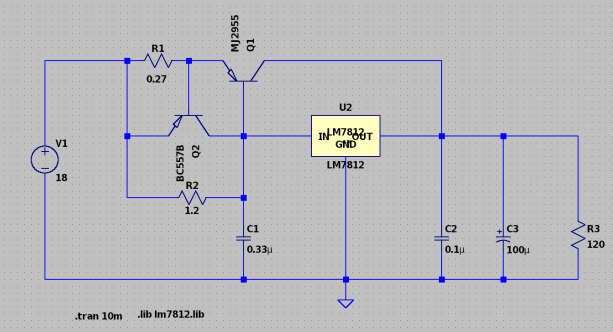
\includegraphics[width=0.88\textwidth]{sch_ltspice.png}
    \caption{Circuito esquemático completo de la fuente regulada con elevador de corriente y limitador de sobrecarga.}
    \label{fig.c5:esquematico}
\end{figure}
